\subsection{Class Diagram}

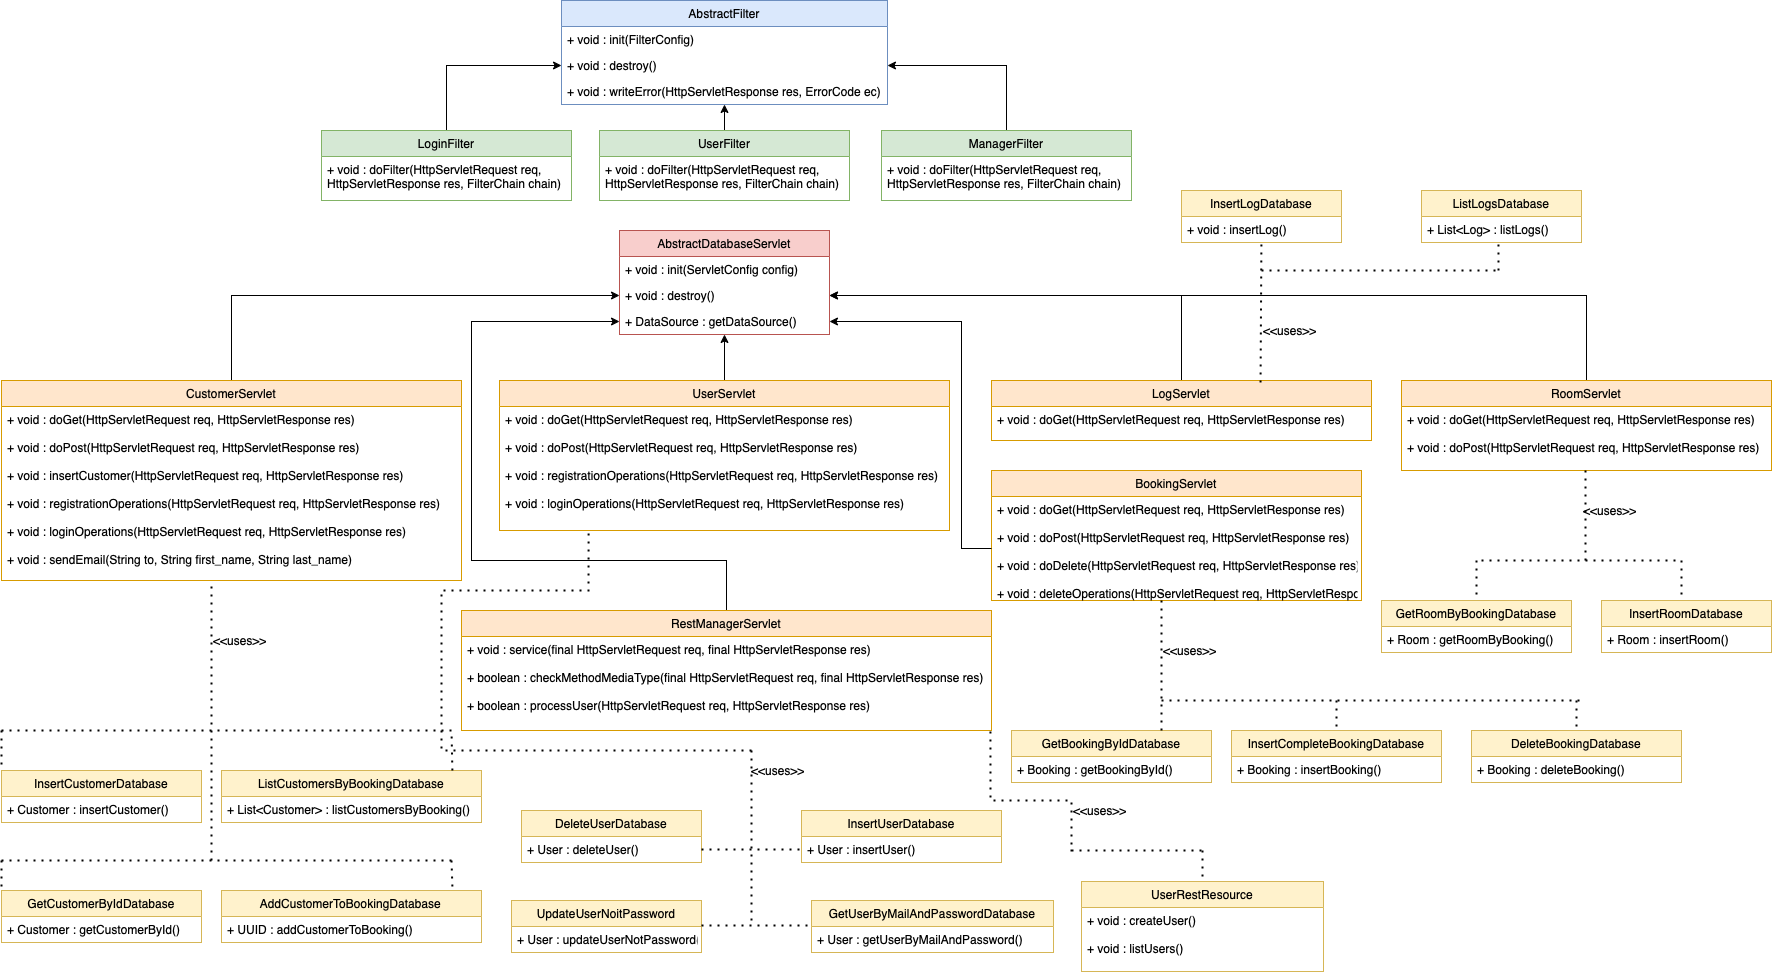
\includegraphics[width=\textwidth]{images/Class_Diagram.png}

The class diagram contains most of the classes used to handle the six different resources; users, customers, bookings, rooms, logging, and manager. All of the resources have their own servlet class which is extended by the AbstractServlet. The AbstractServlet is a subclass of HttpServlet which offers different HTTP requests; doGet, doPost, doPut and doDelete. Whereas the first five resources mentioned have the traditional Java Servlet methods using the Http design, the Manager servlet is based on a traditional REST approach. This servlet mainly parses the URI and determines the type/id the manager wants to interact with. As the request has been processed, it forwards it to the UserRestResource class, which implements the methods to properly handle the resources. All of the servlets uses several Data Access Objects (DAO) which allows us to obtain different resources. 